\documentclass[uplatex,12pt]{jsarticle}
\usepackage[dvipdfmx]{graphicx}
\usepackage{url}
\usepackage{listings,jlisting}
\usepackage{ascmac}
\usepackage{amsmath,amssymb}

%ここからソースコードの表示に関する設定
\lstset{
  basicstyle={\ttfamily},
  identifierstyle={\small},
  commentstyle={\smallitshape},
  keywordstyle={\small\bfseries},
  ndkeywordstyle={\small},
  stringstyle={\small\ttfamily},
  frame={tb},
  breaklines=true,
  columns=[l]{fullflexible},
  numbers=left,
  xrightmargin=0zw,
  xleftmargin=3zw,
  numberstyle={\scriptsize},
  stepnumber=1,
  numbersep=1zw,
  lineskip=-0.5ex
}
%ここまでソースコードの表示に関する設定

\title{知能プログラミング演習II 課題6}
\author{グループ8\\
  29114060 後藤 拓也\\
}
\date{2020年01月04日}

\begin{document}
\maketitle

\paragraph{提出物} rep6
\paragraph{グループ} グループ8

\paragraph{メンバー}
\begin{tabular}{|c|c|c|}
  \hline
  学生番号&氏名&貢献度比率\\
  \hline\hline
  29114003&青山周平&null\\
  \hline
  29114060&後藤拓也&null\\
  \hline
  29114116&増田大輝&null\\
  \hline
  29114142&湯浅範子&null\\
  \hline
  29119016&小中祐希&null\\
  \hline
\end{tabular}



\section{課題の説明}
\begin{description}
\item[必須課題5-1] 目標集合を変えてみたときに,動作が正しくない場合があったかどうか,実行例を示して考察せよ.
また,もしあったならその箇所を修正し,どのように修正したか記せ.
\item[必須課題5-2] 教科書のプログラムでは,オペレータ間の競合解消戦略としてランダムなオペレータ選択を採用している.
これを,効果的な競合解消戦略に改良すべく考察し,実装せよ.
改良の結果,性能がどの程度向上したかを定量的に(つまり数字で)示すこと.
\item[必須課題5-3] 上記のプランニングのプログラムでは,ブロックの属性(たとえば色や形など)を考えていないので,色や形などの属性を扱えるようにせよ.ルールとして表現すること.
例えば色と形の両方を扱えるようにする場合,Aが青い三角形,Bが黄色の四角形,Cが緑の台形であったとする.
その時,色と形を使ってもゴールを指定できるようにする("green on blue" や"blue on box"のように)
\item[必須課題5-4] 上記5-2, 5-3で改良したプランニングシステムのGUIを実装せよ.
ブロック操作の過程をグラフィカルに可視化し,初期状態や目標状態をGUI上で変更できることが望ましい.
\item[発展課題5-5] ブロックワールド内における物理的制約条件をルールとして表現せよ.
例えば,三角錐(pyramid)の上には他のブロックを乗せられない等,その世界における物理的な制約を実現せよ.
\item[発展課題5-6] ユーザが自然言語(日本語や英語など)の命令文によってブロックを操作したり,初期状態/目標状態を変更したりできるようにせよ.
なお,命令文の動詞や語尾を1つの表現に決め打ちするのではなく,多様な表現を許容できることが望ましい.
\item[発展課題5-7] 3次元空間 (実世界) の物理的な挙動を考慮したブロックワールドにおけるプランニングを実現せよ.
なお,物理エンジン等を利用する場合,Java以外の言語のフレームワークを使って実現しても構わない.
\item[発展課題5-8] 教科書3.3節のプランニング手法を応用できそうなブロック操作以外のタスクをグループで話し合い,新たなプランニング課題を自由に設定せよ.
さらに,もし可能であれば,その自己設定課題を解くプランニングシステムを実装せよ.
\end{description}

%%%%%%%%%%%%%%%%%% 必須課題5-2の改良 %%%%%%%%%%%%%%%%%%%%%%%%%%%%%%%%%%%%%%%

\section{必須課題5-2の改良}
\subsection{前回の内容}
前回の課題5-2では, 「Place A on A(存在しない制約)」や「Place B on A(属性を考量した場合の禁止制約)」を改良させるために, 属性クラスであるAttributionsクラスで定義した禁止制約のXonY関係をHashMapに格納し, その条件と現状態のX'onY'関係を照らし合わせるという方法を用いた. オペレータ選択にはランダム選択を用いることで, どんなに適当な状態になっても禁止制約が発動されることを保証するようにした. \\

実行結果は以下のように失敗していた.
\begin{lstlisting}[caption=失敗実行例その1, label=src:No1]
*** GOALS ***[holding B]
**holding B
そのオペレータは実行できません
おすすめのオペレータを使います
**clear ?y3
[clear A, clear B, clear C, ontable A, ontable B, ontable C, ontable pyramid, handEmpty]
*** GOALS ***[holding B]
**holding B
そのオペレータは実行できません
おすすめのオペレータを使います
**clear ?y3
[clear A, clear B, clear C, ontable A, ontable B, ontable C, ontable pyramid, handEmpty]
*** GOALS ***[holding B]
**holding B
そのオペレータは実行できません
おすすめのオペレータを使います
**clear ?y3
...(以下無限に続く)
\end{lstlisting}

問題点としては, 離れた制約がうまく機能していなかったことである. 「B on ?y1」という目標に対して, オペレータ「Place ?x2 on ?y2」によって, 「?x2 = B」と「?y2 = ?y1」となるのはよいが, その後, 「Clear A」と「Clear ?y2」のマッチングを行う際に, 「?y2 = ?y1 = A」となるが, この処理において, 禁止制約(X on Y関係)との関係がうまく取れていなかったのである. 以下の図1を参照してほしい.

% ここに図1を作って説明
\begin{figure}[htbp]
 \begin{center}
  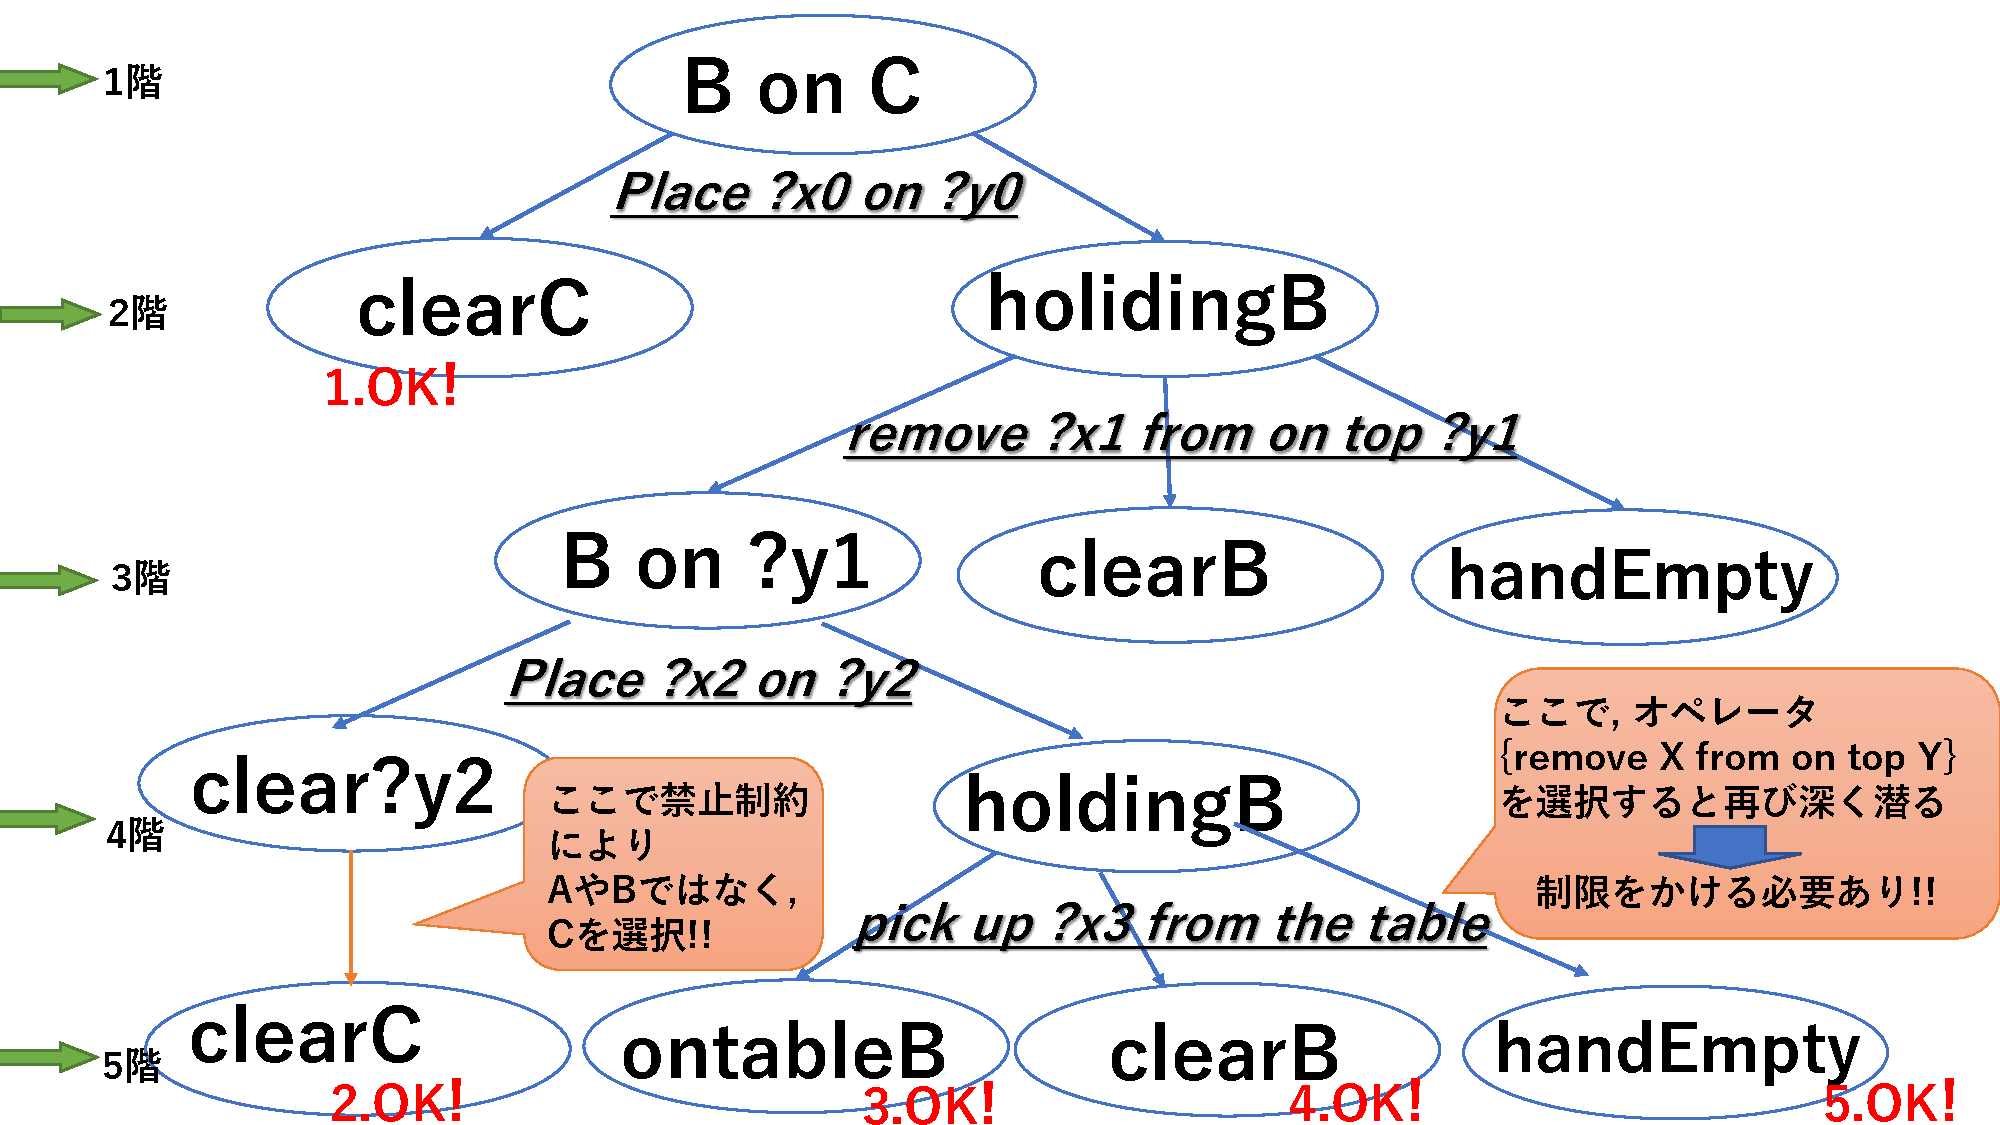
\includegraphics[width = 12cm, pagebox = cropbox, clip]{images/treeContsraction.pdf}
 \end{center}
 \caption[]{plannnigの再帰呼び出しの木構造表現}\label{fig:fig1.1}
\end{figure}

初期設定から与えられる禁止制約:prohibitと, 現在の状態を表す:productKeyOnValueを照らし合わせて, 積み方に制約をかけている. productKeyOnValueには, 「X on Y関係」の目標が生じたときに, 現在問題にしている「X on Y関係」の何がXで何がYかを保存する. これは, 上記で述べたような離れた制約(B on ?y1の後に,Clear ?y2など)にも対応できるようにするためである.

これを実装するにあたり, replaceBufferのタイミングも変更した. 以前のプログラムの内容では, 「?x1 = A」と決まった後で, 「?x2 = A」と制約を加える形をとっていた. それでは, ?x2 = ?x1の対応が取れない.(実装で内容を詳しく説明)\\ % なげやりやね・・・

% 木を図2を用いて表現
また, 木構造を用いてこれらの再帰構造の内容を表現すると図2のようになる.
図2は, 目標「B on C, A on B」における「B on A」を単体目標としたときの再帰構造の様子である. 1階の「B on C」に対して, オペレータ「Place ?x on ?y」のadd部がマッチングし, そのif部が次の目標となり, 1つ深くなり, 2階目へ移行する. その後同様の処理を深さ優先探索として行われる.

ここでポイントになるのは, 「X on Y関係」において, 1階と2階の間で決定される「?x0 on ?y0関係」に対して, 3階で定義される「B on ?y1」関係においては, 4階で決定されるのではなく, 5階で決定される. このように3階で定義されたものが次の階ではなく, 5階で定義される状態を"離れた制約"と呼んでいる. 前回のプログラムではこの点に関してうまくいっていなかった. 今回はこの点を修正した. 実装方法は前回の内容を利用し, 以下のように変更を加えた.

%実装方法の説明
\subsection{実装}
Attribuiteクラスで定義された禁止制約(A on Aなど)をHashMapに格納し, それをPlannerクラスで呼び, Unifierクラスとその情報を共有する. そして現在の「X on Y関係」を保存するHashMap:productKeyOnValueを用いて禁止制約との照らし合わせをする. 以下には前回の実装では失敗していたUnifierクラスでの"禁止制約との照らし合わせによるマッチング"を示す.
\begin{lstlisting}[caption=UnifierクラスのvarMatchingメソッド, label=src:No1]
boolean varMatching(String vartoken, String token) {
 System.out.println("vars="+vars);
 System.out.println("vartoken="+vartoken);
 System.out.println("token="+token);
 if(vars.containsKey(vartoken)) {
   if(token.equals(vars.get(vartoken))) {
	return true;
   }else{
	return false;
   }
 }else{
   /* ココじゃなくて...
   replaceBuffer(vartoken, token);
   if (vars.containsValue(vartoken)) {
      replaceBindings(vartoken, token);
   }
   */
   if(productKeyOnValue != null) {
      //product_KeyValueの数
      for(String str1 : productKeyOnValue.keySet()){	
	   System.out.println("vars="+vars);
	   if(var(productKeyOnValue.get(str1))) {
		for(int num=0; num<prohibit.get(str1).size(); num++) {
		    if(vars.containsKey(productKeyOnValue.get(str1))) {
		     System.out.println(productKeyOnValue.get(str1));
		     if(vars.get(productKeyOnValue.get(str1)).equals(vartoken) & prohibit.get(str1).get(num).equals(token)){
			   System.out.println("禁止制約発動しました.");
			   return false;
			}
		     }
	       }
	     }
      }
   }
  //ココで行います!
  replaceBuffer(vartoken, token);
  if (vars.containsValue(vartoken)) {
	replaceBindings(vartoken, token);
  }
	vars.put(vartoken, token);
  }
  return true;
}
\end{lstlisting}

上記のプログラムでは自分でも何をやっているのかわからなくなるので以下の図2, 図3を参考にしながらプログラムを見ていただきたい.

% 図2 プログラムの内容
\begin{figure}[htpb]
  \centering
    \begin{tabular}{c} 
      \begin{minipage}{0.50\hsize}
        \centering
          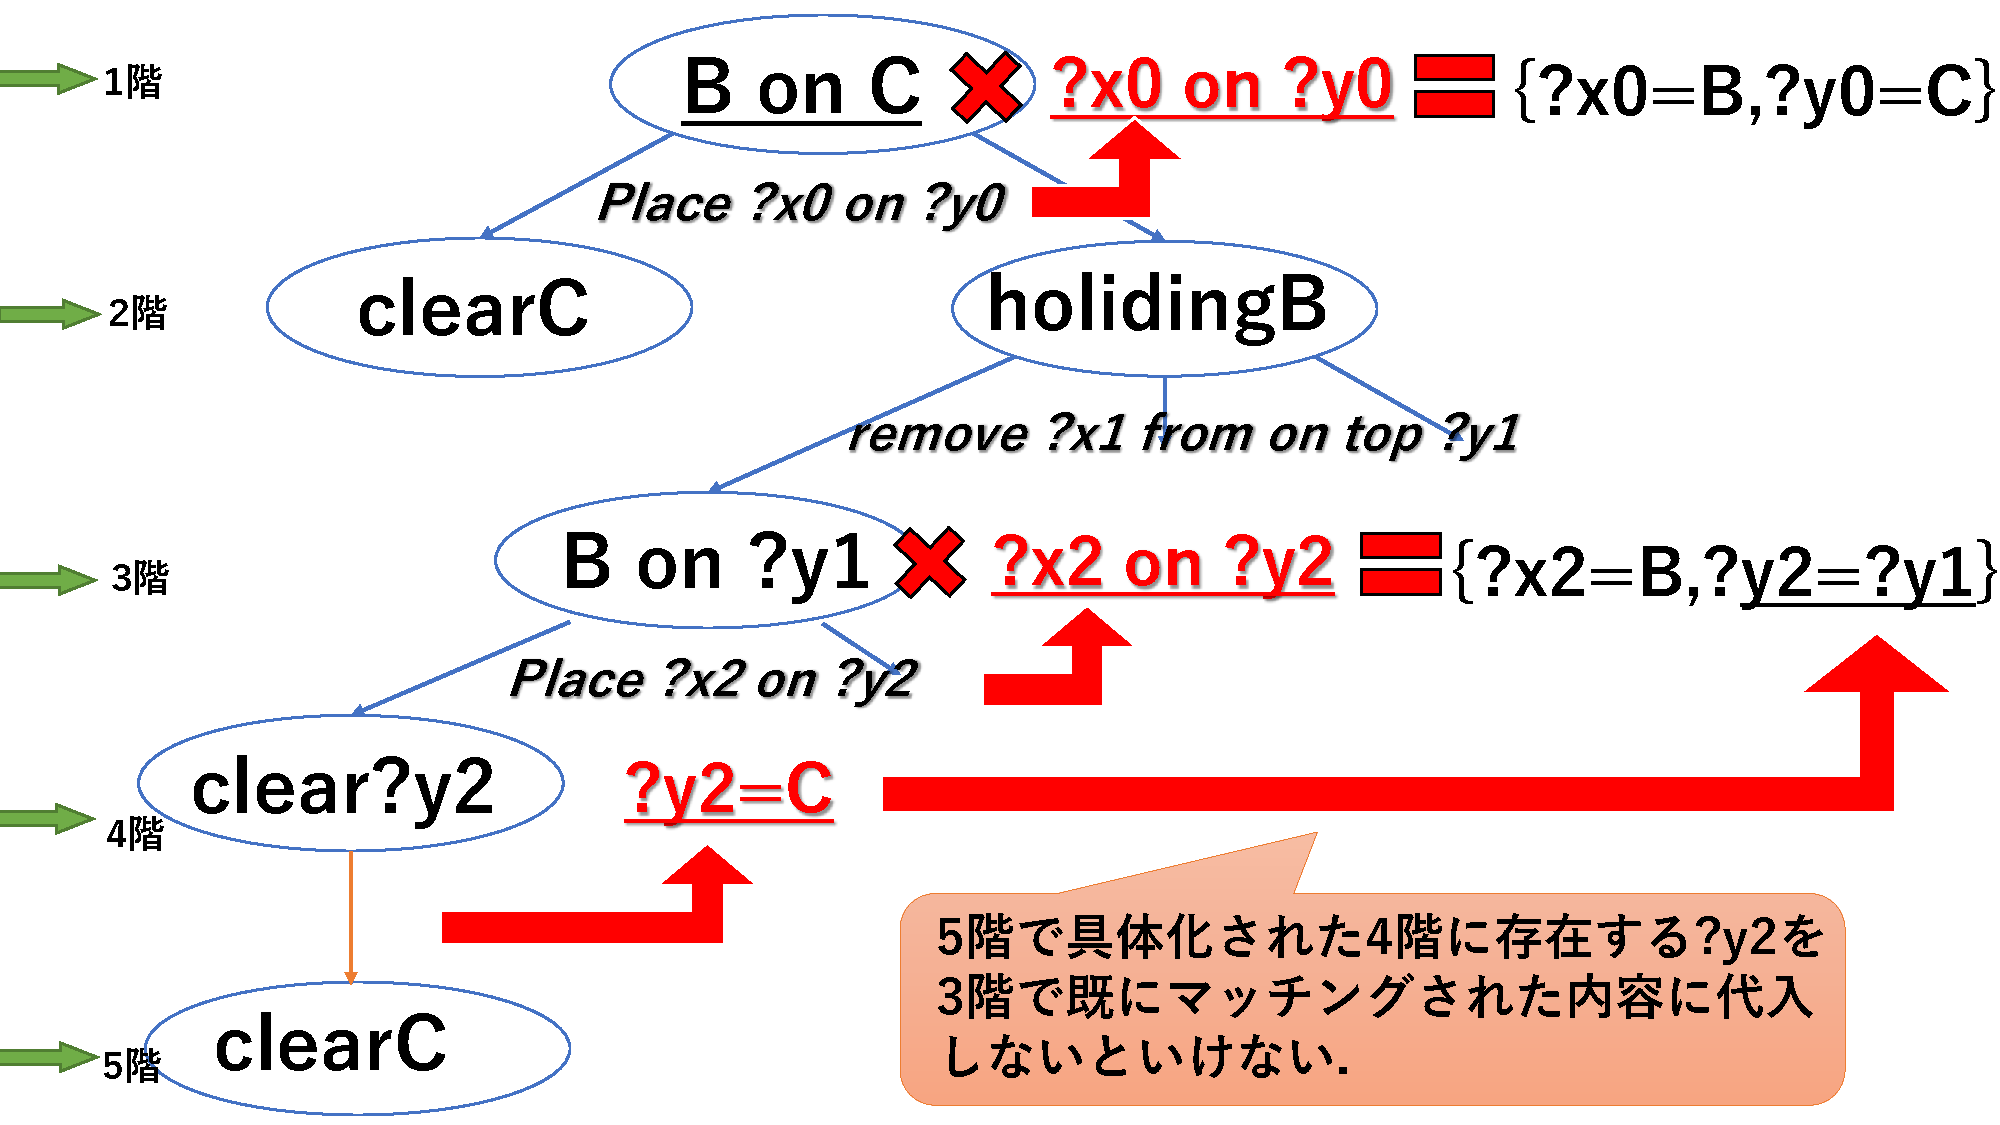
\includegraphics[width = 6.5cm, pagebox = cropbox, clip]
                          {images/treeSupplement.pdf}
                          \caption{階層的な視点}
                          \label{fig:1.3}
      \end{minipage}
 
      \begin{minipage}{0.50\hsize}
        \centering
          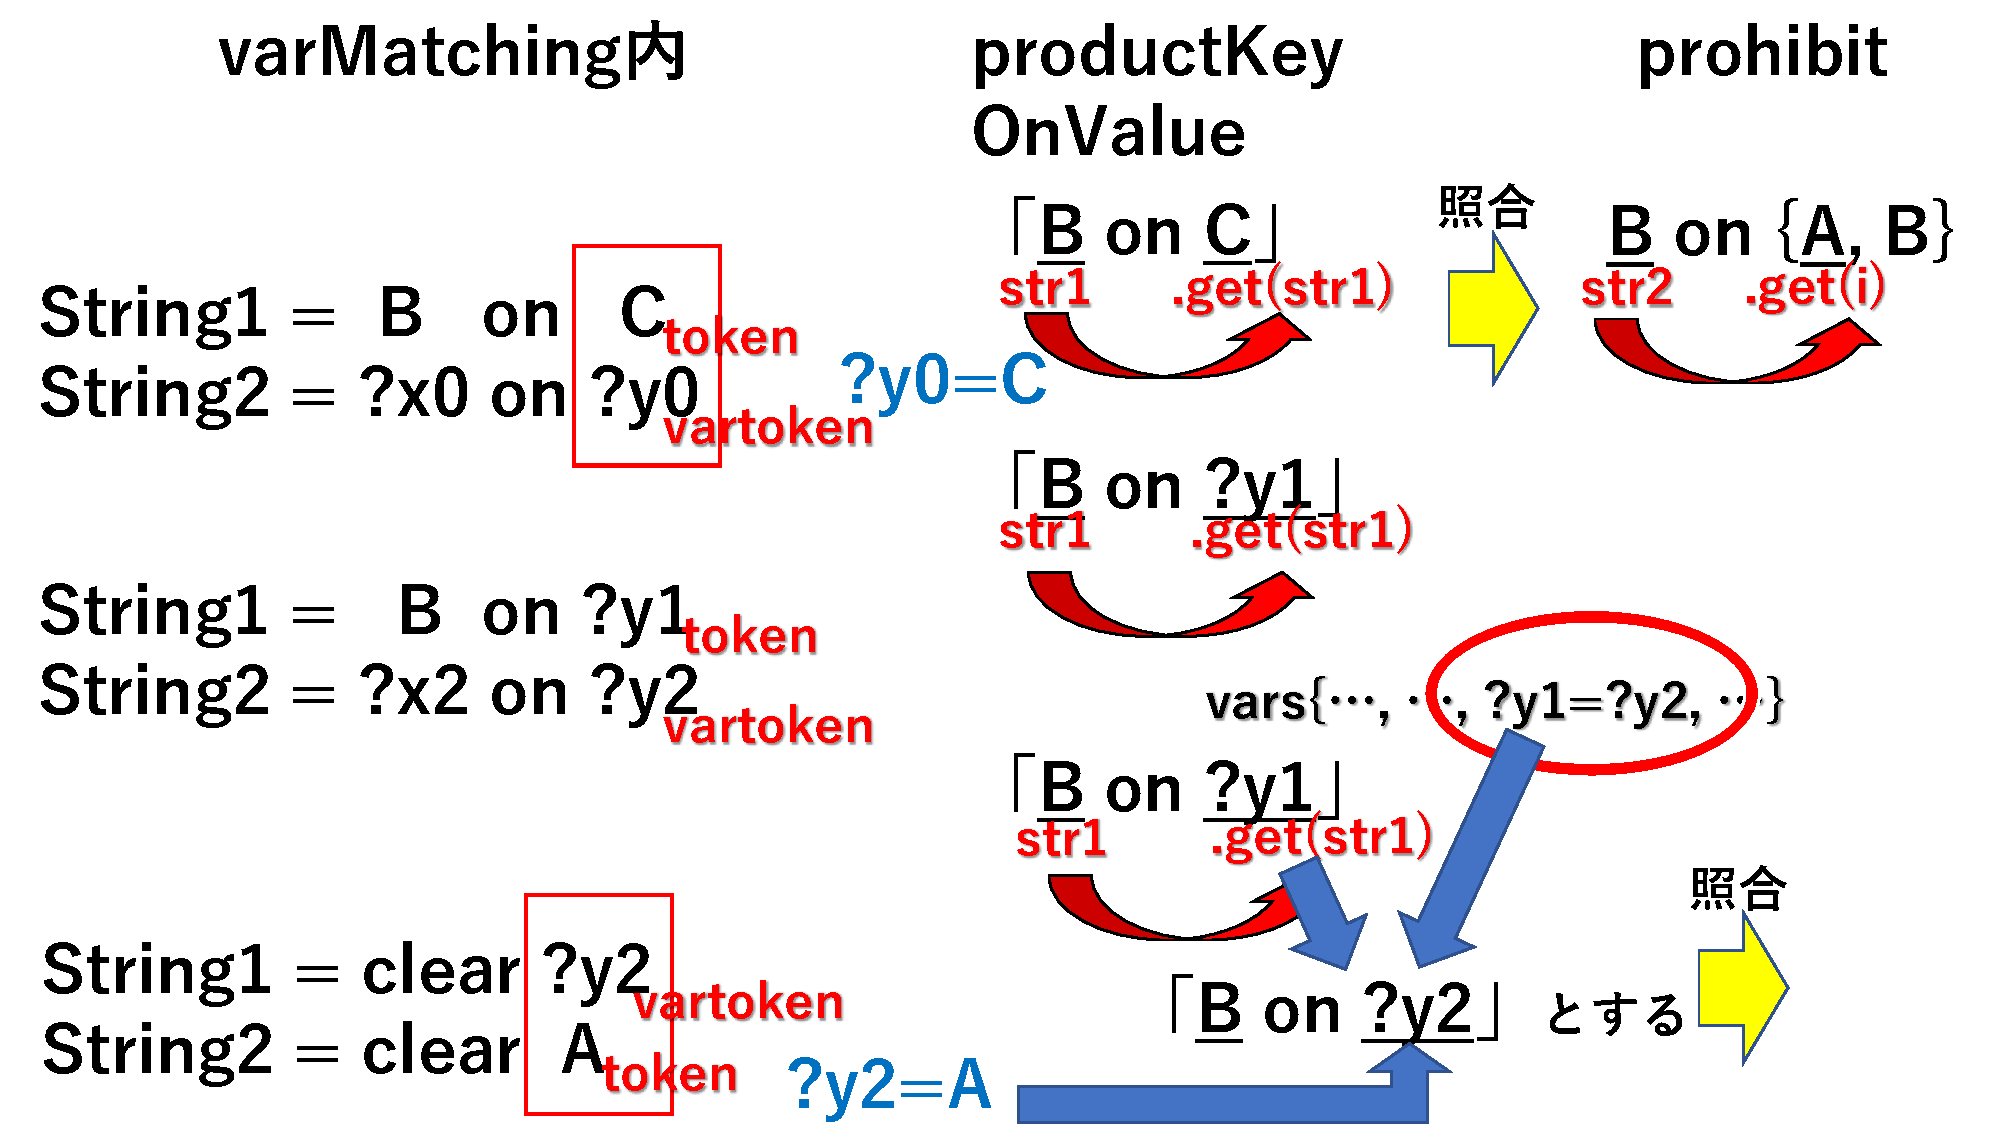
\includegraphics[width = 6.5cm, pagebox = cropbox, clip]
                          {images/varMatching.pdf}
                          \caption{varMatching内の処理内容}
                          \label{fig:1.3}
      \end{minipage} \\ 
    \end{tabular}
\end{figure}     

図2, 3ともに, 「X on Y関係」だけに焦点を絞っている. 図2からは, 「?x0 on ?y0」の場合に2階から1階へのマッチングに対し, 「?x2 on ?y2」の場合は, 5階の「clearC」のCを使って, 3階のマッチングに利用されていることを示している. 図3は, UnifierクラスのVarMatchingメソッド内でのマッチングする2つの文, 現状態XonY関係を示すHashMap:productKeyOnValue, 禁止制約のHashMap:prohibitが示されている. \\

図2の各階のノードが決定された時点で, 図3のproductKeyOnValueにはそのノードの値が代入され, その後, 選択されたオペレータのadd部(X on Yに絞って言及中)とMatchingをする. productKeyOnValueもprohibitも, HashMapなので, 「X on Y」が「Key on Value」の関係で呼び出すことができる. 1,2階間でのマッチング処理は, varMatchingメソッドでマッチングした?x0, ?y0をそのままprohibitの禁止制約と照らし合わせればよいが, 3~5階間でのマッチング処理は, 図2のノードはあくまで, 「B on ?y1」なので, ?y2との関係は「B on ?y1」と「?x2 on ?y2」のマッチングが終わった後に確定される. その関係はハッシュマップ:varsに格納されるので, それを用いて, ノードの「B on ?y1」を「B on ?y2」とする. そして, 4~5階で?y2=Cとマッチングすると, その情報を現状態のノード:productKeyOnValueに代入することで, 「B on A」という関係を生成させる. それと禁止制約を照合することで, 多階層のX on Y関係でも対応できるようにした. プログラムのfor文では, productKeyOnValueのKey値(str1)とVlaue値(.get(str1))を見て, そのKey(str1)に対応する禁止制約のprohibitのVlaue値(.get(str2))をもってきたのち, ifの条件文で, HashMap:varsの{?y1=?y2}関係と禁止制約:prohibitのvalue値を1つずつ照らし合わせる処理をしている.\\

そして以上のvarsの関係[?y1=?y2]の関係を見た後で, ?y2=Cとし, ?y1=Cとするところから, replaceBufferメソッドの呼び出しは, 上記の内容を行った後で実行するようにした. 先にreplaceBufferメソッド呼び出してしまうと, Key:?y1のValue値は?y2となってしまい, 具体化されないまま終わってしまうからである.


\subsection{実行例}
今回の実行においては, 上記の説明を実際に表示させるために, オペレータの選択を自分で選択し, 逐一状況を確認していく.
\begin{lstlisting}[caption=3~5階層のマッチング, label=src:No1]
Place ?x2 on ?y2
addList = [?x2 on ?y2, clear ?x2, handEmpty]
string1=B on ?y1
string2=?x2 on ?y2
productKeyOnValue保存 = {B=?y1}
vars={?y0=C, ?x0=B, ?x1=B}
vartoken=?x2
token=B
productKeyOnValue.get()=?y1
vars={?y0=C, ?x0=B, ?x1=B}
vars={?y0=C, ?x0=B, ?x1=B, ?x2=B}
vartoken=?y1
token=?y2
productKeyOnValue.get()=?y1
vars={?y0=C, ?x0=B, ?x1=B, ?x2=B}
その2
Key = B Value = ?y1
unify成功
オペレータの具体化:Place B on ?y2
*** GOALS ***[clear ?y2, holding B]
**clear ?y2
string1=clear ?y2
string2=clear A
vars={?y0=C, ?x0=B, ?y1=?y2, ?x1=B, ?x2=B}
vartoken=?y2
token=A
productKeyOnValue.get()=?y1
vars={?y0=C, ?x0=B, ?y1=?y2, ?x1=B, ?x2=B}
禁止制約発動しました.
string1=clear ?y2
string2=clear B
vars={?y0=C, ?x0=B, ?y1=?y2, ?x1=B, ?x2=B}
vartoken=?y2
token=B
productKeyOnValue.get()=?y1
vars={?y0=C, ?x0=B, ?y1=?y2, ?x1=B, ?x2=B}
禁止制約発動しました.
string1=clear ?y2
string2=clear C
vars={?y0=C, ?x0=B, ?y1=?y2, ?x1=B, ?x2=B}
vartoken=?y2
token=C
productKeyOnValue.get()=?y1
vars={?y0=C, ?x0=B, ?y1=?y2, ?x1=B, ?x2=B}
theBinding{?y0=C, ?x0=B, ?y1=C, ?x1=B, ?y2=C, ?x2=B}
\end{lstlisting}

「?x2 on ?y2」関係から「clear C」に至るまでの処理を図2,3を参考にしながら見ていただけると, よくわかると思う. 「B on A」という禁止制約が発動され, A, Bではマッチングが行われず, Cのみで成功している. 実際に, 最後のBinding情報では, {?y1=C,...,?y2=C}と正しく行われていることが分かる.

\subsection{考察}
図1の木構造からも分かるように, 問題に上がっていた繰り返しの処理(Place A on B, remove A from on top Bの繰り返し)をなくすには, 「pick up B from the table」を選択するしかないということが分かる.

ただ, 以下の実行結果を見てもらいたい. 最終結果のみを記す.
% 「A on C」という実行結果
\begin{lstlisting}[caption=A on Cが生じてしまう, label=src:No1]
***** This is a plan! *****
pick up B from the table
Place B on C
remove B from on top C
Place B on C
pick up A from the table
Place A on C
remove A from on top C
Place A on B
\end{lstlisting}


確かに, 「A on C」という禁止制約は存在しないが, 既に「B on C」が存在している状況で, 「A on C」とすることは...物理的に不可能である. そのため, 実行中にも, 禁止制約を随時追加していかなければならないことが分かる. ただ, 「B on C」が確定したのちに「A on C」はダメという禁止制約, 「remove B from on top C」を実行された後には, 「A on C」はダメではないので禁止制約から取り除くといった処理を行うのは, また...大変であり, planningの実装に向けては, かなりゲームフィールの制限を強くするしかないことが分かった. "知識システム"の授業で, 新谷先生が「条件を限定した仮想空間を用いないとプログラムに書ききらないよ」と言っていた内容が良く分かった.


\section{必須課題5-2のさらなる改良}
\subsection{序論}
上記では, 禁止制約を「X on Y関係」のHashMapを用いることで解決するアプローチを試みた. その際に, 図1で紹介したが, 「AをとってBの上に置く」, 「AをBから取り除く」, 「AをとってBの上に置く」, 「AをBから取り除く」といった無駄な処理をなくす方法として, オペレータの選択に制限をかける必要があると述べた. 今回はそのプログラムを実装してみる.

\subsection{手法}
図1でもわかるように, 2階で「holdingB」という目標が設定されていて, その後, 4階でも同じ「holdingB」という目標が出てくる. 4階で2階と同じオペレータ(ここでは, remove X from on top Y)を選択したらどんどんと木は深くなる. そのため, planningAGoalメソッドで設定された1つの目標(木構造におけるノード)と, そのノードに対して選択されたオペレータを保存しておき, 繰り返しを防ぐという方法をとる.

\subsection{実装}
Plannerクラスに, 1つの目標(木構造におけるノード)とその時に選択されたオペレータの対応関係を保存するHashMap:goalOpを作成. Keyには目標, Valueにはオペレータのインデント[0~3]を保存する. (オペレータの選択とインデントの関係に関しては, 課題5のレポートを参照してもらいたい.)

\begin{lstlisting}[caption=目標とオペレータの対応関係の保存, label=src:No1]
//Plannerクラス
  HashMap<String, Integer> goalOp;	//Key:単目標/Value:オペレータの番号
//コンストラクタ
  goalOp = new HashMap<String, Integer>();

//planningAGoalメソッド内
  //1.stateリストとの照らし合わせ処理(省略) 
  //2.ノードをKeyとして保存(Value)は未定値
  if(!goalOp.containsKey(theGoal)) {
    goalOp.put(theGoal, -1);
  }
  //3.operatorの選択(ランダム)
  int randInt = Math.abs(rand.nextInt())\%operators.size();
  Operator op = (Operator)operators.get(randInt);
  cPoint = randInt;
  //4-1.選択したオペレータの実行(一部省略)
  Operator anOperator = rename((Operator) operators.get(cPoint));
  for (int j = 0; j < addList.size(); j++) {
    Unifier unification = new Unifier();
    if(unification.unify(theGoal, (String) addList.get(j), theBinding, attributions.keyValueProhibit, p_productKeyOnValue)) {
      //5.一度は選択されていたら,break
      if(goalOp.get(theGoal) == cPoint) {
        System.out.println("breakします");
	  break;
      }
      //6.breakしなかったら, 保存する
      goalOp.put(theGoal, cPoint);
      System.out.println("goalOp"+goalOp);
	...
  //4-2.選択されたオペレータが実行されない場合,
  for (int i = 0; i < operators.size(); i++) {
    if(i != cPoint) {
    anOperator = rename((Operator) operators.get(i));
    addList = (ArrayList<String>) anOperator.getAddList();
    for (int j = 0; j < addList.size(); j++) {
      Unifier unification = new Unifier();
	if(unification.unify(theGoal, (String) addList.get(j), theBinding, attributions.keyValueProhibit, p_productKeyOnValue)) {
     //5.既にその目標に対してオペレータが選択されていたら,
	  if(goalOp.get(theGoal) == i) {
             System.out.println("breakします");
		break;
          }
     //6.保存する
	goalOp.put(theGoal, i);
	System.out.println("goalOp"+goalOp);
	...
\end{lstlisting}

選択したオペレータが実際に実行されるか, それとも別のオペレータが実行されるかに関しては, 課題5のレポートを参考にしてもらいたい.

planningAGoalメソッドが実行されたら, まず, HashMap:goalOpにその目標がKeyとして設定されていない場合は, Valueを-1としておく. それ以前にすでにその目標がKeyとして保存されていたら, -1の初期化は行わない. その後, 実際に, オペレータのadd部とunifyをしていき, 成功したら, そのオペレータのインデントをgoalOpのValueに加える(上書き保存する). すでにその目標に対して, 以前実行されたオペレータがあり, 保存されていたら(つまり-1ではなかったら), 別のオペレータを探すためにfor文をbreakし, 下の"選択されたオペレータ以外のオペレータの実行" へ移動する. そこで, 一度も選択されていないオペレータだったら, そのオペレータを実行する.

\subsection{実行結果}
\begin{lstlisting}[caption=goalOpによって制約される , label=src:No1]
[B on C, A on B]
*** GOALS ***[B on C, A on B]
**B on C
Place ?x0 on ?y0
goalOp{B on C=0}
*** GOALS ***[clear C, holding B]
**clear C
theBinding{?y0=C, ?x0=B}
*** GOALS ***[holding B]
**holding B
remove ?x1 from on top ?y1
goalOp{holding B=1, B on C=0}
オペレータの具体化:remove B from on top ?y1
*** GOALS ***[B on ?y1, clear B, handEmpty]
**B on ?y1
Place ?x2 on ?y2
goalOp{holding B=1, B on C=0, B on ?y1=0}
オペレータの具体化:Place B on ?y2
*** GOALS ***[clear ?y2, holding B]
**clear ?y2
theBinding{?y0=C, ?x0=B, ?y1=C, ?x1=B, ?y2=C, ?x2=B}
*** GOALS ***[holding B]
**holding B
Place ?x3 on ?y3
そのオペレータは実行できません
remove ?x4 from on top ?y4
breakします
pick up ?x5 from the table
オペレータの具体化:pick up B from the table
*** GOALS ***[ontable B, clear B, handEmpty]
**ontable B
theBinding{?y0=C, ?x0=B, ?y1=C, ?x1=B, ?y2=C, ?x2=B, ?x4=B, ?x5=B}
*** GOALS ***[clear B, handEmpty]
**clear B
theBinding{?y0=C, ?x0=B, ?y1=C, ?x1=B, ?y2=C, ?x2=B, ?x4=B, ?x5=B}
*** GOALS ***[handEmpty]
**handEmpty
theBinding{?y0=C, ?x0=B, ?y1=C, ?x1=B, ?y2=C, ?x2=B, ?x4=B, ?x5=B}
Success !
Success !
Success !
...
\end{lstlisting}

「holdingB」が2回目の目標として設定された際に, 「Place ?x3 on ?y3」のオペレータを選択しているが, add文には「holdingX」が存在しないので, 次のオペレータを探す. すると, 「remove ?x4 from on top ?y4」が選択されるが, goalOpにすでに{holding B=1}と保存されているので, インデント1のremoveオペレータは実行されない. その後, 「pick up ?x5 from the table」が実行され, 成功していることが分かる.

\subsection{考察}
このプログラムにより, オペレータの選択をランダムにしても, 無駄な処理(AをBの上に置いて, AをBから取り除いて, またAをBの上において...など)はなくなった. 完璧なプログラムかといえば, 結局, 「Place A on C」という前に述べた"物理的に不可能な置き方"が残ってしまったので, 残念である. また, "机に置いてある3つの積み木(A, B, C)を順に上に積んでいく"という処理しかできなくなり, 汎用性がなくなってしまった. 本当は積み木が4つになって, 初期状態がどうであれ, 最終的な目標状態がどうであれ, 適切なオペレータ選択ができればよかったが, なかなか難しい...

\section{感想}
前回の内容が行き当たりばったりのプログラムであったので, 今回の修繕にとても時間を要した. 具体的なエラーに対して対処しても次のエラーが生じて, 全てのエラーを直すのに本当に時間がかかってしまった. 汎用性の高いプログラムを作るには, もっとさまざまなパターンを頭の中でイメージしないといけないので, やはり難しい.

再帰構造のプログラムの処理の流れを把握するには, やはり木構造を用いるのが一番わかりやすいということが分かった. 木構造を用いることができれば, 2年生の前期に大囿先生から学んだ"知能処理学"の内容や, 加藤先生から学んだ"知識表現と推論"がとても生きてくることが分かり, 今までの総復習をしながら今回の課題に取り組むことができてよかった. \\
先生に最後にお願いしたいこととしては, ぜひ次の世代の子にも, 今回自分が取り組んだPlannningの木構造表現方法を勧めてほしい. 欲を言えば, これを一つの課題にしてもらえると, バックトラックを用いたプランニングの全体概要が面白いようにわかると思う. この3.3章のプランニングの実行過程に関しては, "知能プログラミング入門"の教科書に詳しくのっていなかったため, プランニングの内部構造をしっかり理解できているのが, グループの中でも僕だけで, 今回の課題もだいぶしんどかった. 木構造で表現することで, もう少し,グループ内で, プランニングの処理の流れを共有し, 役割分担しやすくなると思う. さらに言えば, 今回自分は時間がなかったのでできなかったが, プログラム実行しながら, この木構造を表現するGUIがあると, もっと直観的にわかりやすくなるとも思った. これは来年度の発展課題にしてもらえると面白いかもしれない.\\

最後に, この知能系演習を通して, たくさんの経験を積むことができた. ここまで6つの課題を最後まで一緒に取り組んでくれたグループのメンバーには本当に感謝する. また, 今まで教えてくださった知能系の先生方にも感謝し申し上げます.

 "知識"とは"データの関連"であり, "推論"とは, "知識を利用して結論を導くこと"である. この3年間で人工知能の本質を経験することができた. ありがとうございました.

%%%%%%%%%%%%%%%%%% 参考文献 %%%%%%%%%%%%%%%%%%%%%%%%%%%%%%%%%%%%%%%
\begin{thebibliography}{99}
\bibitem{notty} Javaによる知能プログラミング入門 --著:新谷 虎松 \\
\bibitem{notty} 知識システムの実装基礎 --著:新谷 虎松 \\
\bibitem{notty} 人工知能の基礎知識 --著:太原 育夫 \\
\bibitem{notty} LATEX2ε 美文書作成入門 --著:奥村 晴彦 \\
\end{thebibliography}

\end{document}